\question \textbf{Bitvectors}
Proof the statement on slide 2059 is true:
\begin{equation}
\begin{pmatrix}
b\\c
\end{pmatrix}
\cdot
\begin{pmatrix}
b\\c'
\end{pmatrix}
\leq
\begin{pmatrix}
2\cdot b\\c + c'
\end{pmatrix}
\end{equation}



\begin{solution}

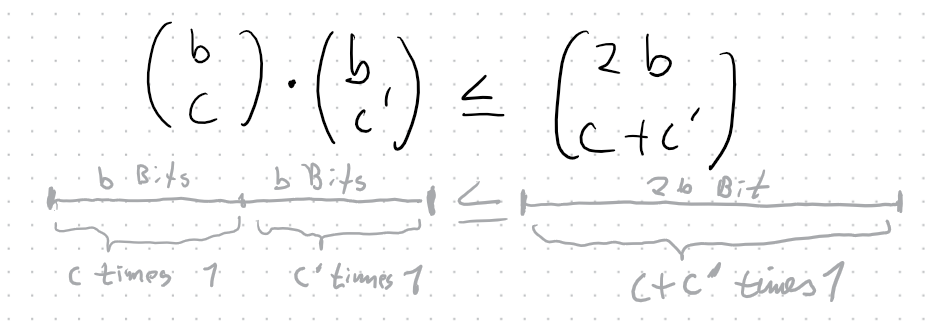
\includegraphics[width=0.5\linewidth]{task_3/a3.png}

The left side of the inequality is the number of possible $2b$ long bitvectors with $c$ 1s in the left half and $c'$ 1s in the right half. The right side of the inequality is the number of possible $2b$ long bitvectors in with $c+c'$ 1s in total. So the inequality is obviously true, because the bitvectors with $c$ 1s in the left and $c'$ 1s in the right half are a subset of the bitvectors with $c+c'$ 1s in total.

To prove that the statement on slide 2059 is true, we can use the definition of the binomial coefficient to expand the left-hand side and right-hand side of the equation. The binomial coefficient is defined as follows:

\begin{equation}
\begin{pmatrix}
b\\c
\end{pmatrix}
= \frac{b!}{c!(b - c)!}
\end{equation}

Therefore, the left-hand side of the equation can be written as:

\begin{equation}
\begin{pmatrix}
b\\c
\end{pmatrix}
\cdot
\begin{pmatrix}
b\\c'
\end{pmatrix}
= \frac{b!}{c!(b - c)!} \cdot \frac{b!}{c'!(b - c')!}
\end{equation}

We can simplify this expression by canceling out the common factors in the numerator and denominator:

\begin{equation}
\frac{b!}{c!(b - c)!} \cdot \frac{b!}{c'!(b - c')!}
= \frac{b! \cdot b!}{c! \cdot (b - c)! \cdot c'! \cdot (b - c')!}
= \frac{(b!)^2}{c! \cdot (b - c)! \cdot c'! \cdot (b - c')!}
\end{equation}

Next, we can expand the right-hand side of the equation using the definition of the binomial coefficient:

\begin{equation}
\begin{pmatrix}
2 \cdot b\\c + c'
\end{pmatrix}
= \frac{(2 \cdot b)!}{(c + c')!(2 \cdot b - c - c')!}
\end{equation}

To prove that the left-hand side is less than or equal to the right-hand side, we need to show that the numerator of the left-hand side is less than or equal to the numerator of the right-hand side, and that the denominator of the left-hand side is less than or equal to the denominator of the right-hand side.

First, we can see that the numerator of the left-hand side is $(b!)^2$, while the numerator of the right-hand side is $(2 \cdot b!)^2$. Since $(b!)^2 \leq (2 \cdot b!)^2$, the numerator of the left-hand side is less than or equal to the numerator of the right-hand side.

Next, we can see that the denominator of the left-hand side is $c! \cdot (b - c)! \cdot c'! \cdot (b - c')!$, while the denominator of the right-hand side is $(c + c')! \cdot (2 \cdot b - c - c')!$. We can prove that the denominator of the left-hand side is less than or equal to the denominator of the right-hand side by using the fact that $a! \leq b!$ for all positive integers $a$ and $b$ such that $a \leq b$.

In particular







\end{solution}